\section{La dinámica analítica para el caso $\mcU=\textsc{SWAP}$}

Utilizando la expresión (\ref{eq:MaxEntZ}), se puede pasar tanto a $\varrho_{max}$ como a $\varrho_{max}$ a través de la aplicación de grano grueso. El resultado $\CG{\varrho_{max}}$ corresponde al estado grueso inicial, pero en términos de $\lambda$. Así:
\begin{equation}
\rho(0)=\frac{1}{Z}\CG{\varrho_{max}}=\frac{e^{-\lambda_{3}p\sigma_{z}}}{Z_{1}}+(1-p)\frac{e^{-\lambda_{3}(1-p)\sigma_{z}}}{Z_{2}},
\end{equation}
\begin{equation}
\rho(t=1)=\frac{1}{Z}\CG{S\varrho_{max} S}=p\frac{e^{-\lambda_{3}(1-p)\sigma_{z}}}{Z_{2}}+(1-p)\frac{e^{-\lambda_{3}p\sigma_{z}}}{Z_{1}}.
\end{equation}
Tanto el estado grueso inicial como el final son estados que, en la base de Pauli, su única componente no nula es la $z$. Esto significa que podemos relacionar ambas coordenadas a través de un coeficiente de compresión:
\begin{equation}\label{eq:SWAPFactor}
            \frac{r_{z}(1)}{r_{z}(0)}=\left(\frac{2 \sinh (\lambda )}{\sinh (\lambda )+(1-2 p) \sinh (\lambda -2 \lambda  p)}-1\right)
\end{equation}
Esto puede comprobarse en los resultados numéricos mostrados en la figura \ref{fig:factornnum}.
\begin{figure}[h!]
\centering
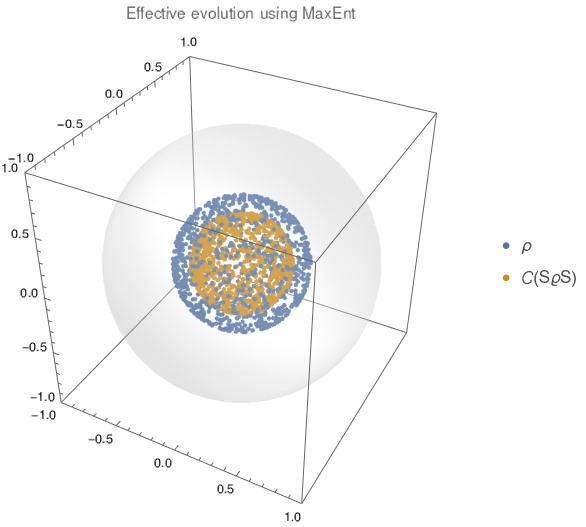
\includegraphics[width=0.6\linewidth]{maxent/figures/MaxEnt_SWAP_t0vst1_n=5000_z=0.5_p=0.3_beta=150_delta=0.6.png}
\caption{Apreciación del factor de compresión \notaAd{aquí está bueno comparar la diferencia radial numérica con el factor analítico}}
\label{fig:factornnum}
\end{figure}

\subsection{Caso $p=\frac{1}{2}$}

Aunque es posible repetir todas las cuentas desde la contrucción del estado de máxima entropía, haciendo $p=\frac{1}{2}$, basta con ver que el factor (\eqref{eq:SWAPFactor}) es $1$ en dicho caso. Así, todos los estado gruesos son puntos fijos bajo una evolución subyacente SWAP con aplicación de grano grueso con parámetro $p=\frac{1}{2}$.
